\documentclass{beamer}

\usepackage{graphicx}
\graphicspath{{images/}} %Setting the graphicspath

%\usetheme{Copenhagen}
%\usetheme{AnnArbor}
\usetheme[outer/progressbar=foot]%,outer/numbering=none]
{metropolis}

%build gantt chart
\usepackage{styles/gantt}
%disable numbering in math equations
\usepackage{amsmath}
%draw plots in latex
\usepackage{pgfplots}
%draw figures and gannt charts
\usepackage{tikz}
%draw horizontal  rules in tables
\usepackage{booktabs}
%enable multipage table header repeat
\usepackage{xtab}
%enable set width columns in xtabular
\usepackage{array}
%enable caption in xtabular tables
\usepackage{caption}
%enable \Verb command inside tables
\usepackage{fvextra}
%allow appendix slides 
\usepackage{appendixnumberbeamer}
%print license Disclaimer using \ccbysa command
\usepackage[scale=2]{ccicons}
%add a space unless the macro is followed by punctuation
\usepackage{xspace}
%drawing algorithms 2 packages
\usepackage{algorithm}
\usepackage{algorithmic} 
%output code listings
\usepackage{listings}
%\usepackage{adjustbox}
%recommended fonts for metropolis theme
\usepackage[sfdefault]{FiraSans}

%\usepackage[T1]{fontenc}
%latin modern family of fonts
%\usepackage{lmodern}
%provide optional arguments to the \includegraphics command
%\usepackage{graphicx}
%\usepackage{xcolor}

%create a box named \codebox to store code listings
\newsavebox{\codebox}% For storing  code listings
%create \themename command to point to word metropolis
\newcommand{\themename}{\textbf{\textsc{metropolis}}\xspace}
%create \defcolor command to point to color of gantt bar
\newcommand{\defcolor}{red}
%create \flow command to point to rightleftharpoons character
\newcommand{\flow}{\rightleftharpoons}

%\definecolor{Purple}{HTML}{911146}
%\setbeamercolor{frametitle}{bg=Purple}
%\definecolor{Alternate}{HTML}{3366cc}
%\setbeamercolor{frametitle}{bg=Alternate}

%change fonts to other alternatives
%\usepackage[sfdefault]{sourcesanspro}

%---------------

\title{Creating Polished Presentations}
\date{West New York, \today.}
\author{Valerii Klymchuk \\ www.voklymchuk.com}
\email{jpkumquat@consortium.net}
\institute{Centre for Modern Templates}


\begin{document}
\maketitle


\begin{frame}[allowframebreaks]{Outline}
	\medskip
	\tableofcontents
\end{frame}

\begin{frame}[standout]
	Thanks for your attention.
	Pay attention here...
\end{frame}

 %---------------
\section{Introduction} 

\begin{frame}
	This is going to be a normal paragraph in our introduction.
	
	
		Some intro stuff
		\begin{block}{Observation}
			This is a very important piece of information.
		\end{block}
		Some other stuff ...


\end{frame}


\begin{frame}{Blocks}
	Three different block environments are pre-defined and may be styled with an
	optional background color.
	
	\begin{columns}[T,onlytextwidth]
		\column{0.5\textwidth}
		\begin{block}{Default}
			Block content.
		\end{block}
		
		\begin{alertblock}{Alert}
			Block content.
		\end{alertblock}
		
		\begin{exampleblock}{Example}
			Block content.
		\end{exampleblock}
		
		\column{0.5\textwidth}
		
		\metroset{block=fill}
		
		\begin{block}{Default}
			Block content.
		\end{block}
		
		\begin{alertblock}{Alert}
			Block content.
		\end{alertblock}
		
		\begin{exampleblock}{Example}
			Block content.
		\end{exampleblock}
		
	\end{columns}
\end{frame}


\section{Tables, figures and subfiles}\label{sec:background}
\subsection{Tables and Figures}

\begin{frame}
To insert a figure, you can use the TeXnicecenter menus. 
\begin{figure}
	\centering
	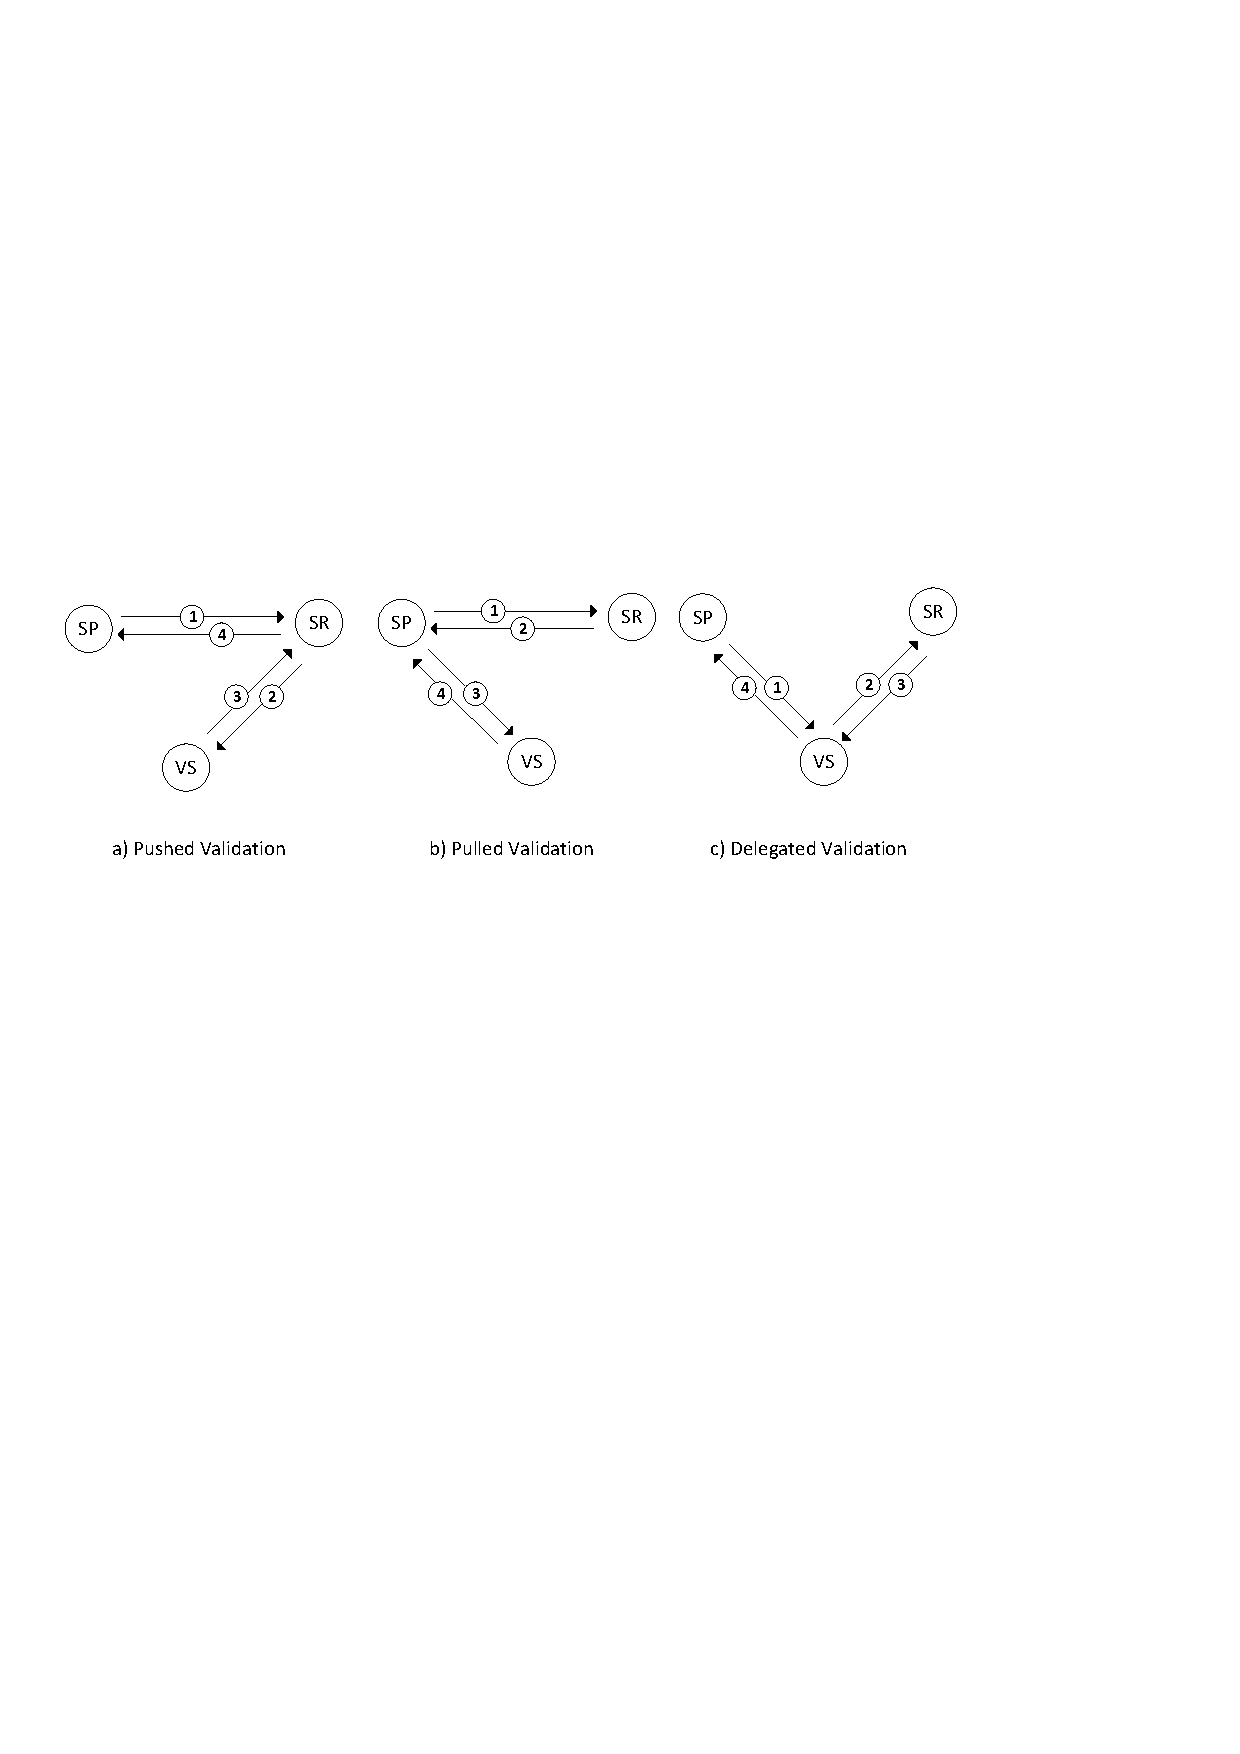
\includegraphics[width=1.00\linewidth]{att-models-base.pdf}
	\caption{My First Figure}
	\label{fig:att-models-base}
\end{figure}
\end{frame}

\begin{frame}{Tikspictures}
	\begin{figure}
		%\resizebox{\linewidth}{!}{
		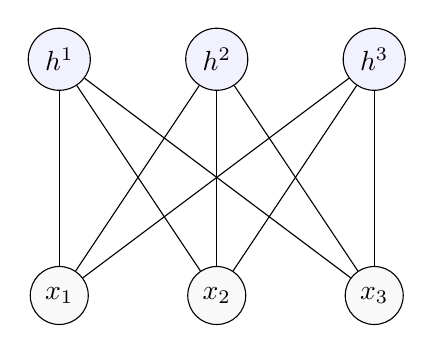
\begin{tikzpicture}	
		\tikzset{
			hcirc/.style={
				draw, circle, fill=blue!5
			},
			xcirc/.style={
				hcirc, fill=gray!5
			}
		}
		
		\foreach \i in {1, ..., 3}{
			\node [hcirc] (h\i) at (\i*2,3) {$h^\i$};
		}
		
		\foreach \i in {1, ..., 3}{
			\node [xcirc] (x\i) at (\i*2,0) {$x_\i$};
		}
		
		\foreach \i in {1, ..., 3}{
			\foreach \v in {1, ..., 3}{
				\path (h\i) edge [draw] (x\v);
			}
		}
		\end{tikzpicture}
		%}	
		\caption{M1} \label{fig:M1}
	\end{figure}
\end{frame}

\begin{frame}[fragile,allowframebreaks]{Multipage Xtabular table}
\begin{table}
	\tablecaption
	{
		Sample multipage table with repeating header 
	}
	\label{tab:MyFirstTable}
	\tablefirsthead{
		\toprule  & \bf document class  &\bf bibliography style &   \\ \midrule
	}
	\tablehead{
		\\
		\multicolumn{4}{c}{\text{\tablename~\thetable{}  continued }} \\
		\midrule &\bf document class &\bf bibliography style &  \\ \midrule
	}

	\begin{xtabular}{
			p{0.25\linewidth}
			p{0.27\linewidth}
			p{0.17\linewidth}
			m{0.15\linewidth}
		}
		Institute of Electrical and Electronics Engineers &\Verb|IEEEtran| & \Verb|IEEEtran|& \raisebox{-0.5\totalheight}{
\includegraphics[width=1\linewidth]{ieee.png}}\\ \midrule
		Association for Computing Machinery & \Verb|sig-alternate|  & \Verb|plain| & \raisebox{-0.5\totalheight}{
\includegraphics[width=1\linewidth]{acm.jpeg}}   \\ \midrule
		Lecture Notes in Computer Science& \Verb|llncs|& \Verb|lllncs|& \raisebox{-0.5\totalheight}{
\includegraphics[width=1\linewidth]{llncs.png}}  \\ \midrule
		General & \Verb|article|  & \Verb|plain|  &  \\ 
		
		\bottomrule
	\end{xtabular}
\end{table}
\end{frame}

\begin{frame}{Gant charts}
	\begin{figure}
		\centering
		\resizebox{\linewidth}{!}
		{
			\begin{gantt}[drawledgerline=true, xunitlength=\linewidth/25]{11}{24}
				% vertical, horizontal 'boxes'
				\begin{ganttitle}
					\numtitle{2020}{3}{2020}{10}
					% start, label, width 
					\numtitle{2021}{1}{2021}{12}
					\numtitle{2022}{1}{2022}{2}
				\end{ganttitle}
				\begin{ganttitle}
					\numtitle{3}{1}{12}{1}
					% start, skip, end, width 
					\numtitle{1}{1}{12}{1}
					\numtitle{1}{1}{2}{1}
				\end{ganttitle}
				\ganttmilestone{Proposal Defense}{0} % Label, position
				%=======================================
				\ganttgroup{Background Study}{0}{6} % start, width 
				\ganttbar[color=\defcolor]{Android Security}{0}{3}
				\ganttbarcon[color=\defcolor]{Code Analysis}{3}{2}
				\ganttbarcon[color=\defcolor]{Policy Mechanisms}{5}{1}
				\ganttmilestonecon{Literature Review Complete}{6}
				% notice the 'con' at the end -- for continue 
				%=======================================
				\ganttbarcon[color=\defcolor]{
					\textbf{Formal Specification} % can format labels!
				}{6}{6}
				\ganttmilestonecon{Spec Document}{12}
				%=======================================
				\ganttbar[color=blue]{Thesis and Paper Writing}{0}{24}
			\end{gantt}
			
		}	
		\caption{My First Gantt}\label{fig:gantt-1}
		
	\end{figure}
\end{frame}

\begin{frame}
\subsection{Cross-references} 
Some text here that wants to refer to Table~\ref{tab:MyFirstTable}. You can also refer to the Figure~\ref{fig:att-models-base}. When you want to refer to a previous section, you can use the \Verb|\ref| command again. Section~\ref{sec:background}.%Section~\ref{sec:drilled-down}. 

\subsection{Sub section through input command}
This comes from a separate file. Notice that we have this subsection included in the Navigator.  

\end{frame}

\begin{frame}{Algorithms}
\begin{algorithm}[H]
	\begin{algorithmic}[2]
		\REQUIRE{Randomly populated array}
		\ENSURE{Sorted array}
		\IF{$i\leq0$}
		\STATE $i\gets1$
		\ELSE 
		\IF{$i\geq0$} \label{line:impline}
		\FOR{$j=0$ \TO $10$}
		\STATE blah()
		\STATE carryOutSomeProcessing() \label{line:mostimp}
		\ENDFOR
		\ENDIF
		\ENDIF
		\RETURN i
	\end{algorithmic}
	\caption{My First Simple Algorithm}
	\label{algo:first}
\end{algorithm}
\end{frame}
\begin{frame}
And of course, we can refer to the algorithm using \Verb|\ref|: See Algorithm~\ref{algo:first} but the good thing is we can also refer to a specific line e.g. Line~\ref{line:impline} or Line~\ref{line:mostimp}.
\end{frame}


\section{Displaying Mathematics}

\begin{frame}
\LaTeX\ is extremely powerful when it comes to typesetting mathematics. It's one of the core strengths of this system. 

There are two ways of displaying maths. One is \emph{inline} and the other is \emph{display} format -- in which the whole math sits on its own set of lines.

\subsection{Inline Mode}
We are going to insert a mathematics equation inline here using a pair of \$ signs: $E=mc^2$   . As you can see, the display (such as line spacing) does not get messed up by the mathematics as it does with word processing softwares. 
\end{frame}

\begin{frame}
\subsection{Display Mode}
We can also display equations in their own set of lines. To do this, we can use the equation environment. 

\begin{equation}\label{eq:emc}
E=mc^2
\end{equation}

As you can see, \LaTeX\ inserts the equation number automatically. We can refer to it using the \Verb|\ref| command just as we referred to sections, figures and tables. (E.g. Equation~\ref{eq:emc}.) To get rid of the equation number, simply use the \emph{star variant} of the equation environment. (For this, you need the \texttt{amsmath} package.)

\begin{equation*}
E=mc^2
\end{equation*}
\end{frame}

Alternatively, we can use the shorthand keys \Verb|\[| and \Verb|\]|
\[
E=mc^2
\]


\LaTeX\ has many builtin features and you can get many more easily. Here, we'll see some of these features: 

Addition, subtraction, multiplication and division: 

\[
x+2 - 25 \times 35 \div 98 
\]

Superscripts and subscripts: 

\[ x^2  \]
\[ x_{(i)} \]

Summation, union, intersection, big-union, integral: 

\[ \sum_{i=1}^{n}{i^2} \]
\[ x \cup y \cap z \]
\[ \bigcup_{i=1}^{n}{x_i} \]
\[ \int_0^n{x^2} \]


\begin{frame}
Fractions, brackets, square root: 

\[ \frac{x}{y} \]
\[ \frac{\sum_i{x^2}}{\int_0^n{x^2}} \]
\[ \sqrt{\frac{\sqrt{36}} {x^5}} \]

\[ 2 \times \left( \frac{34}{\frac{124}{356}}    \right)  \]
\end{frame}

\begin{frame}
Greek letters: 

\[
\alpha + \beta + \gamma^* + \Sigma + \Theta + 2_\epsilon 
\]

Matrices and vectors. For this, you need to include the \texttt{amsmath} package and then use the \texttt{bmatrix} or \texttt{pmatrix} environment: 

\[
\begin{pmatrix}
\frac{a}{44} & b \\ 
c & \sqrt{d} 	
\end{pmatrix}
\]

Accents: 

\[ \hat{x} \]
\[ \hat{\imath} \] 
\[ \dot{x} \]
\end{frame}

\begin{frame}
See the \texttt{Math} menu in the IDE for other operations. You can refer to ``Short Math Guide for \LaTeX'' for a lot more examples. 
\end{frame}



\section{Code Listings and Using Symbols}

\begin{frame}
You might come across situations where you need to find new symbols. For this, you can refer to the ``The Comprehensive \LaTeX Symbols List''.  

\[ x \rightleftharpoons  y \]


(Optional) Since this is a long command, we might want to create a shortcut using the \Verb|\newcommand| command in the preamble. This also allows us to later change the symbol without having to change the equations. 
\[ x \flow y \]
\end{frame}




\lstset{language=[LaTeX]tex}
\lstset{caption=Some \LaTeX Code}
\begin{lrbox}{\codebox}
\begin{lstlisting}[frame=single]{}
\lstset{language=[LaTeX]tex}
\lstset{caption=Some \LaTeX Code}
\begin{lrbox}{\codebox}
  \begin{lstlisting*}[frame=single]{}
     \begin{frame}
	  \end{frame}
  \end{lstlisting*}
\end{lrbox}
\begin{frame}{\LaTeX Code}
  \usebox{\codebox}
\end{frame}	
\end{lstlisting}
\end{lrbox}
\begin{frame}{\LaTeX Code}
	\usebox{\codebox}
\end{frame}



\lstset{language=c++}
\lstset{caption=Some C++ Code}
\begin{lrbox}{\codebox}
	\begin{lstlisting}[frame=single, basicstyle=\ttfamily]{}
	for(i = 0; i < 10; i++){
	// increment the pointer
	*p++ = i;
	}
	\end{lstlisting}
\end{lrbox}
\begin{frame}{C++ Code}
	\usebox{\codebox}
\end{frame}




\begin{frame}{Line plots}
	\begin{figure}
		\begin{tikzpicture}
		\begin{axis}[
		mlineplot,
		width=0.9\textwidth,
		height=6cm,
		]
		
		\addplot {sin(deg(x))};
		\addplot+[samples=100] {sin(deg(2*x))};
		
		\end{axis}
		\end{tikzpicture}
	\end{figure}
\end{frame}





\begin{frame}{Bar charts}
	\begin{figure}
		\begin{tikzpicture}
		\begin{axis}[
		mbarplot,
		xlabel={Foo},
		ylabel={Bar},
		width=0.9\textwidth,
		height=6cm,
		]
		
		\addplot plot coordinates {(1, 20) (2, 25) (3, 22.4) (4, 12.4)};
		\addplot plot coordinates {(1, 18) (2, 24) (3, 23.5) (4, 13.2)};
		\addplot plot coordinates {(1, 10) (2, 19) (3, 25) (4, 15.2)};
		
		\legend{lorem, ipsum, dolor}
		
		\end{axis}
		\end{tikzpicture}
	\end{figure}
\end{frame}






{%
	\setbeamertemplate{frame footer}{My custom footer}
	\begin{frame}[fragile]{Frame footer}
		\themename defines a custom beamer template to add a text to the footer. It can be set via
		\begin{verbatim}\setbeamertemplate{frame footer}{My custom footer}\end{verbatim}
	\end{frame}
}

\begin{frame}{References}
	Some references to showcase~\cite{knuth92,ConcreteMath,Simpson,Er01,greenwade93}
\end{frame}

\section{Conclusion}

\begin{frame}{Summary}
	
	Get the source of this theme and the demo presentation from
	
	\begin{center}\url{github.com/voklymchuk/latex_templates}\end{center}
	
	The theme \emph{itself} is licensed under a
	\href{http://creativecommons.org/licenses/by-sa/4.0/}{Creative Commons
		Attribution-ShareAlike 4.0 International License}.
	
	\begin{center}\ccbysa\end{center}
	
\end{frame}

\begin{frame}[standout]
	Questions?
\end{frame}

\appendix

\begin{frame}[fragile]{Backup slides}
	Sometimes, it is useful to add slides at the end of your presentation to
	refer to during audience questions.
	
	The best way to do this is to include the \verb|appendixnumberbeamer|
	package in your preamble and call \verb|\appendix| before your backup slides.
	
	\themename will automatically turn off slide numbering and progress bars for
	slides in the appendix.
\end{frame}


\begin{frame}[allowframebreaks]{References}
	
	\bibliography{bibfile}
	\bibliographystyle{abbrv}
	
\end{frame}

\end{document}

